\documentclass[11pt,compress,t,notes=noshow, xcolor=table]{beamer}
\documentclass[11pt,compress,t,notes=noshow, xcolor=table]{beamer}
\usepackage[]{graphicx}\usepackage[]{color}
% maxwidth is the original width if it is less than linewidth
% otherwise use linewidth (to make sure the graphics do not exceed the margin)
\makeatletter
\def\maxwidth{ %
  \ifdim\Gin@nat@width>\linewidth
    \linewidth
  \else
    \Gin@nat@width
  \fi
}
\makeatother

\definecolor{fgcolor}{rgb}{0.345, 0.345, 0.345}
\newcommand{\hlnum}[1]{\textcolor[rgb]{0.686,0.059,0.569}{#1}}%
\newcommand{\hlstr}[1]{\textcolor[rgb]{0.192,0.494,0.8}{#1}}%
\newcommand{\hlcom}[1]{\textcolor[rgb]{0.678,0.584,0.686}{\textit{#1}}}%
\newcommand{\hlopt}[1]{\textcolor[rgb]{0,0,0}{#1}}%
\newcommand{\hlstd}[1]{\textcolor[rgb]{0.345,0.345,0.345}{#1}}%
\newcommand{\hlkwa}[1]{\textcolor[rgb]{0.161,0.373,0.58}{\textbf{#1}}}%
\newcommand{\hlkwb}[1]{\textcolor[rgb]{0.69,0.353,0.396}{#1}}%
\newcommand{\hlkwc}[1]{\textcolor[rgb]{0.333,0.667,0.333}{#1}}%
\newcommand{\hlkwd}[1]{\textcolor[rgb]{0.737,0.353,0.396}{\textbf{#1}}}%
\let\hlipl\hlkwb

\usepackage{framed}
\makeatletter
\newenvironment{kframe}{%
 \def\at@end@of@kframe{}%
 \ifinner\ifhmode%
  \def\at@end@of@kframe{\end{minipage}}%
  \begin{minipage}{\columnwidth}%
 \fi\fi%
 \def\FrameCommand##1{\hskip\@totalleftmargin \hskip-\fboxsep
 \colorbox{shadecolor}{##1}\hskip-\fboxsep
     % There is no \\@totalrightmargin, so:
     \hskip-\linewidth \hskip-\@totalleftmargin \hskip\columnwidth}%
 \MakeFramed {\advance\hsize-\width
   \@totalleftmargin\z@ \linewidth\hsize
   \@setminipage}}%
 {\par\unskip\endMakeFramed%
 \at@end@of@kframe}
\makeatother

\definecolor{shadecolor}{rgb}{.97, .97, .97}
\definecolor{messagecolor}{rgb}{0, 0, 0}
\definecolor{warningcolor}{rgb}{1, 0, 1}
\definecolor{errorcolor}{rgb}{1, 0, 0}
\newenvironment{knitrout}{}{} % an empty environment to be redefined in TeX

\usepackage{alltt}
\newcommand{\SweaveOpts}[1]{}  % do not interfere with LaTeX
\newcommand{\SweaveInput}[1]{} % because they are not real TeX commands
\newcommand{\Sexpr}[1]{}       % will only be parsed by R
\newcommand{\xmark}{\ding{55}}%


\usepackage[english]{babel}
\usepackage[utf8]{inputenc}

\usepackage{dsfont}
\usepackage{verbatim}
\usepackage{amsmath}
\usepackage{amsfonts}
\usepackage{amssymb}
\usepackage{bm}
\usepackage{csquotes}
\usepackage{multirow}
\usepackage{longtable}
\usepackage{booktabs}
\usepackage{enumerate}
\usepackage[absolute,overlay]{textpos}
\usepackage{psfrag}
\usepackage{algorithm}
\usepackage{algpseudocode}
\usepackage{eqnarray}
\usepackage{arydshln}
\usepackage{tabularx}
\usepackage{placeins}
\usepackage{tikz}
\usepackage{setspace}
\usepackage{colortbl}
\usepackage{mathtools}
\usepackage{wrapfig}
\usepackage{bm}
\usepackage{amsmath}
\usepackage{pifont}

\usetikzlibrary{shapes,arrows,automata,positioning,calc,chains,trees, shadows}
\tikzset{
  %Define standard arrow tip
  >=stealth',
  %Define style for boxes
  punkt/.style={
    rectangle,
    rounded corners,
    draw=black, very thick,
    text width=6.5em,
    minimum height=2em,
    text centered},
  % Define arrow style
  pil/.style={
    ->,
    thick,
    shorten <=2pt,
    shorten >=2pt,}
}

\usepackage{subfig}

% Defines macros and environments
\usepackage{../../style/lmu-lecture}


\let\code=\texttt
\let\proglang=\textsf

\setkeys{Gin}{width=0.9\textwidth}

\setbeamertemplate{frametitle}{\expandafter\uppercase\expandafter\insertframetitle}

% This file is included in slides and exercises

% Rarely used fontstyle for R packages, used only in 
% - forests/slides-forests-benchmark.tex
% - exercises/single-exercises/methods_l_1.Rnw
% - slides/cart/attic/slides_extra_trees.Rnw
\newcommand{\pkg}[1]{{\fontseries{b}\selectfont #1}}

% Spacing helpers, used often (mostly in exercises for \dlz)
\newcommand{\lz}{\vspace{0.5cm}} % vertical space (used often in slides)
\newcommand{\dlz}{\vspace{1cm}}  % double vertical space (used often in exercises, never in slides)
\newcommand{\oneliner}[1] % Oneliner for important statements, used e.g. in iml, algods
{\begin{block}{}\begin{center}\begin{Large}#1\end{Large}\end{center}\end{block}}

% Don't know if this is used or needed, remove?
% textcolor that works in mathmode
% https://tex.stackexchange.com/a/261480
% Used e.g. in forests/slides-forests-bagging.tex
% [...] \textcolor{blue}{\tfrac{1}{M}\sum^M_{m} [...]
% \makeatletter
% \renewcommand*{\@textcolor}[3]{%
%   \protect\leavevmode
%   \begingroup
%     \color#1{#2}#3%
%   \endgroup
% }
% \makeatother





% dependencies: amsmath, amssymb, dsfont
% math spaces
\ifdefined\N
\renewcommand{\N}{\mathds{N}} % N, naturals
\else \newcommand{\N}{\mathds{N}} \fi
\newcommand{\Z}{\mathds{Z}} % Z, integers
\newcommand{\Q}{\mathds{Q}} % Q, rationals
\newcommand{\R}{\mathds{R}} % R, reals
\ifdefined\C
\renewcommand{\C}{\mathds{C}} % C, complex
\else \newcommand{\C}{\mathds{C}} \fi
\newcommand{\continuous}{\mathcal{C}} % C, space of continuous functions
\newcommand{\M}{\mathcal{M}} % machine numbers
\newcommand{\epsm}{\epsilon_m} % maximum error

% counting / finite sets
\newcommand{\setzo}{\{0, 1\}} % set 0, 1
\newcommand{\setmp}{\{-1, +1\}} % set -1, 1
\newcommand{\unitint}{[0, 1]} % unit interval

% basic math stuff
\newcommand{\xt}{\tilde x} % x tilde
\newcommand{\argmin}{\mathop{\mathrm{arg\,min}}} % argmin
\newcommand{\argmax}{\mathop{\mathrm{arg\,max}}} % argmax
\newcommand{\argminlim}{\argmin\limits} % argmin with limits
\newcommand{\argmaxlim}{\argmax\limits} % argmax with limits
\newcommand{\sign}{\operatorname{sign}} % sign, signum
\newcommand{\I}{\mathbb{I}} % I, indicator
\newcommand{\order}{\mathcal{O}} % O, order
\newcommand{\bigO}{\mathcal{O}} % Big-O Landau
\newcommand{\littleo}{{o}} % Little-o Landau
\newcommand{\pd}[2]{\frac{\partial{#1}}{\partial #2}} % partial derivative
\newcommand{\floorlr}[1]{\left\lfloor #1 \right\rfloor} % floor
\newcommand{\ceillr}[1]{\left\lceil #1 \right\rceil} % ceiling
\newcommand{\indep}{\perp \!\!\! \perp} % independence symbol

% sums and products
\newcommand{\sumin}{\sum\limits_{i=1}^n} % summation from i=1 to n
\newcommand{\sumim}{\sum\limits_{i=1}^m} % summation from i=1 to m
\newcommand{\sumjn}{\sum\limits_{j=1}^n} % summation from j=1 to p
\newcommand{\sumjp}{\sum\limits_{j=1}^p} % summation from j=1 to p
\newcommand{\sumik}{\sum\limits_{i=1}^k} % summation from i=1 to k
\newcommand{\sumkg}{\sum\limits_{k=1}^g} % summation from k=1 to g
\newcommand{\sumjg}{\sum\limits_{j=1}^g} % summation from j=1 to g
\newcommand{\summM}{\sum\limits_{m=1}^M} % summation from m=1 to M
\newcommand{\meanin}{\frac{1}{n} \sum\limits_{i=1}^n} % mean from i=1 to n
\newcommand{\meanim}{\frac{1}{m} \sum\limits_{i=1}^m} % mean from i=1 to n
\newcommand{\meankg}{\frac{1}{g} \sum\limits_{k=1}^g} % mean from k=1 to g
\newcommand{\meanmM}{\frac{1}{M} \sum\limits_{m=1}^M} % mean from m=1 to M
\newcommand{\prodin}{\prod\limits_{i=1}^n} % product from i=1 to n
\newcommand{\prodkg}{\prod\limits_{k=1}^g} % product from k=1 to g
\newcommand{\prodjp}{\prod\limits_{j=1}^p} % product from j=1 to p

% linear algebra
\newcommand{\one}{\bm{1}} % 1, unitvector
\newcommand{\zero}{\mathbf{0}} % 0-vector
\newcommand{\id}{\bm{I}} % I, identity
\newcommand{\diag}{\operatorname{diag}} % diag, diagonal
\newcommand{\trace}{\operatorname{tr}} % tr, trace
\newcommand{\spn}{\operatorname{span}} % span
\newcommand{\scp}[2]{\left\langle #1, #2 \right\rangle} % <.,.>, scalarproduct
\newcommand{\mat}[1]{\begin{pmatrix} #1 \end{pmatrix}} % short pmatrix command
\newcommand{\Amat}{\mathbf{A}} % matrix A
\newcommand{\Deltab}{\mathbf{\Delta}} % error term for vectors

% basic probability + stats
\renewcommand{\P}{\mathds{P}} % P, probability
\newcommand{\E}{\mathds{E}} % E, expectation
\newcommand{\var}{\mathsf{Var}} % Var, variance
\newcommand{\cov}{\mathsf{Cov}} % Cov, covariance
\newcommand{\corr}{\mathsf{Corr}} % Corr, correlation
\newcommand{\normal}{\mathcal{N}} % N of the normal distribution
\newcommand{\iid}{\overset{i.i.d}{\sim}} % dist with i.i.d superscript
\newcommand{\distas}[1]{\overset{#1}{\sim}} % ... is distributed as ...

% machine learning
\newcommand{\Xspace}{\mathcal{X}} % X, input space
\newcommand{\Yspace}{\mathcal{Y}} % Y, output space
\newcommand{\Zspace}{\mathcal{Z}} % Z, space of sampled datapoints
\newcommand{\nset}{\{1, \ldots, n\}} % set from 1 to n
\newcommand{\pset}{\{1, \ldots, p\}} % set from 1 to p
\newcommand{\gset}{\{1, \ldots, g\}} % set from 1 to g
\newcommand{\Pxy}{\mathbb{P}_{xy}} % P_xy
\newcommand{\Exy}{\mathbb{E}_{xy}} % E_xy: Expectation over random variables xy
\newcommand{\xv}{\mathbf{x}} % vector x (bold)
\newcommand{\xtil}{\tilde{\mathbf{x}}} % vector x-tilde (bold)
\newcommand{\yv}{\mathbf{y}} % vector y (bold)
\newcommand{\xy}{(\xv, y)} % observation (x, y)
\newcommand{\xvec}{\left(x_1, \ldots, x_p\right)^\top} % (x1, ..., xp)
\newcommand{\Xmat}{\mathbf{X}} % Design matrix
\newcommand{\allDatasets}{\mathds{D}} % The set of all datasets
\newcommand{\allDatasetsn}{\mathds{D}_n}  % The set of all datasets of size n
\newcommand{\D}{\mathcal{D}} % D, data
\newcommand{\Dn}{\D_n} % D_n, data of size n
\newcommand{\Dtrain}{\mathcal{D}_{\text{train}}} % D_train, training set
\newcommand{\Dtest}{\mathcal{D}_{\text{test}}} % D_test, test set
\newcommand{\xyi}[1][i]{\left(\xv^{(#1)}, y^{(#1)}\right)} % (x^i, y^i), i-th observation
\newcommand{\Dset}{\left( \xyi[1], \ldots, \xyi[n]\right)} % {(x1,y1)), ..., (xn,yn)}, data
\newcommand{\defAllDatasetsn}{(\Xspace \times \Yspace)^n} % Def. of the set of all datasets of size n
\newcommand{\defAllDatasets}{\bigcup_{n \in \N}(\Xspace \times \Yspace)^n} % Def. of the set of all datasets
\newcommand{\xdat}{\left\{ \xv^{(1)}, \ldots, \xv^{(n)}\right\}} % {x1, ..., xn}, input data
\newcommand{\ydat}{\left\{ \yv^{(1)}, \ldots, \yv^{(n)}\right\}} % {y1, ..., yn}, input data
\newcommand{\yvec}{\left(y^{(1)}, \hdots, y^{(n)}\right)^\top} % (y1, ..., yn), vector of outcomes
\newcommand{\greekxi}{\xi} % Greek letter xi
\renewcommand{\xi}[1][i]{\xv^{(#1)}} % x^i, i-th observed value of x
\newcommand{\yi}[1][i]{y^{(#1)}} % y^i, i-th observed value of y
\newcommand{\xivec}{\left(x^{(i)}_1, \ldots, x^{(i)}_p\right)^\top} % (x1^i, ..., xp^i), i-th observation vector
\newcommand{\xj}{\xv_j} % x_j, j-th feature
\newcommand{\xjvec}{\left(x^{(1)}_j, \ldots, x^{(n)}_j\right)^\top} % (x^1_j, ..., x^n_j), j-th feature vector
\newcommand{\phiv}{\mathbf{\phi}} % Basis transformation function phi
\newcommand{\phixi}{\mathbf{\phi}^{(i)}} % Basis transformation of xi: phi^i := phi(xi)

%%%%%% ml - models general
\newcommand{\lamv}{\bm{\lambda}} % lambda vector, hyperconfiguration vector
\newcommand{\Lam}{\bm{\Lambda}}	 % Lambda, space of all hpos
% Inducer / Inducing algorithm
\newcommand{\preimageInducer}{\left(\defAllDatasets\right)\times\Lam} % Set of all datasets times the hyperparameter space
\newcommand{\preimageInducerShort}{\allDatasets\times\Lam} % Set of all datasets times the hyperparameter space
% Inducer / Inducing algorithm
\newcommand{\ind}{\mathcal{I}} % Inducer, inducing algorithm, learning algorithm

% continuous prediction function f
\newcommand{\ftrue}{f_{\text{true}}}  % True underlying function (if a statistical model is assumed)
\newcommand{\ftruex}{\ftrue(\xv)} % True underlying function (if a statistical model is assumed)
\newcommand{\fx}{f(\xv)} % f(x), continuous prediction function
\newcommand{\fdomains}{f: \Xspace \rightarrow \R^g} % f with domain and co-domain
\newcommand{\Hspace}{\mathcal{H}} % hypothesis space where f is from
\newcommand{\fbayes}{f^{\ast}} % Bayes-optimal model
\newcommand{\fxbayes}{f^{\ast}(\xv)} % Bayes-optimal model
\newcommand{\fkx}[1][k]{f_{#1}(\xv)} % f_j(x), discriminant component function
\newcommand{\fh}{\hat{f}} % f hat, estimated prediction function
\newcommand{\fxh}{\fh(\xv)} % fhat(x)
\newcommand{\fxt}{f(\xv ~|~ \thetav)} % f(x | theta)
\newcommand{\fxi}{f\left(\xv^{(i)}\right)} % f(x^(i))
\newcommand{\fxih}{\hat{f}\left(\xv^{(i)}\right)} % f(x^(i))
\newcommand{\fxit}{f\left(\xv^{(i)} ~|~ \thetav\right)} % f(x^(i) | theta)
\newcommand{\fhD}{\fh_{\D}} % fhat_D, estimate of f based on D
\newcommand{\fhDtrain}{\fh_{\Dtrain}} % fhat_Dtrain, estimate of f based on D
\newcommand{\fhDnlam}{\fh_{\Dn, \lamv}} %model learned on Dn with hp lambda
\newcommand{\fhDlam}{\fh_{\D, \lamv}} %model learned on D with hp lambda
\newcommand{\fhDnlams}{\fh_{\Dn, \lamv^\ast}} %model learned on Dn with optimal hp lambda
\newcommand{\fhDlams}{\fh_{\D, \lamv^\ast}} %model learned on D with optimal hp lambda

% discrete prediction function h
\newcommand{\hx}{h(\xv)} % h(x), discrete prediction function
\newcommand{\hh}{\hat{h}} % h hat
\newcommand{\hxh}{\hat{h}(\xv)} % hhat(x)
\newcommand{\hxt}{h(\xv | \thetav)} % h(x | theta)
\newcommand{\hxi}{h\left(\xi\right)} % h(x^(i))
\newcommand{\hxit}{h\left(\xi ~|~ \thetav\right)} % h(x^(i) | theta)
\newcommand{\hbayes}{h^{\ast}} % Bayes-optimal classification model
\newcommand{\hxbayes}{h^{\ast}(\xv)} % Bayes-optimal classification model

% yhat
\newcommand{\yh}{\hat{y}} % yhat for prediction of target
\newcommand{\yih}{\hat{y}^{(i)}} % yhat^(i) for prediction of ith targiet
\newcommand{\resi}{\yi- \yih}

% theta
\newcommand{\thetah}{\hat{\theta}} % theta hat
\newcommand{\thetav}{\bm{\theta}} % theta vector
\newcommand{\thetavh}{\bm{\hat\theta}} % theta vector hat
\newcommand{\thetat}[1][t]{\thetav^{[#1]}} % theta^[t] in optimization
\newcommand{\thetatn}[1][t]{\thetav^{[#1 +1]}} % theta^[t+1] in optimization
\newcommand{\thetahDnlam}{\thetavh_{\Dn, \lamv}} %theta learned on Dn with hp lambda
\newcommand{\thetahDlam}{\thetavh_{\D, \lamv}} %theta learned on D with hp lambda
\newcommand{\mint}{\min_{\thetav \in \Theta}} % min problem theta
\newcommand{\argmint}{\argmin_{\thetav \in \Theta}} % argmin theta

% densities + probabilities
% pdf of x
\newcommand{\pdf}{p} % p
\newcommand{\pdfx}{p(\xv)} % p(x)
\newcommand{\pixt}{\pi(\xv~|~ \thetav)} % pi(x|theta), pdf of x given theta
\newcommand{\pixit}[1][i]{\pi\left(\xi[#1] ~|~ \thetav\right)} % pi(x^i|theta), pdf of x given theta
\newcommand{\pixii}[1][i]{\pi\left(\xi[#1]\right)} % pi(x^i), pdf of i-th x

% pdf of (x, y)
\newcommand{\pdfxy}{p(\xv,y)} % p(x, y)
\newcommand{\pdfxyt}{p(\xv, y ~|~ \thetav)} % p(x, y | theta)
\newcommand{\pdfxyit}{p\left(\xi, \yi ~|~ \thetav\right)} % p(x^(i), y^(i) | theta)

% pdf of x given y
\newcommand{\pdfxyk}[1][k]{p(\xv | y= #1)} % p(x | y = k)
\newcommand{\lpdfxyk}[1][k]{\log p(\xv | y= #1)} % log p(x | y = k)
\newcommand{\pdfxiyk}[1][k]{p\left(\xi | y= #1 \right)} % p(x^i | y = k)

% prior probabilities
\newcommand{\pik}[1][k]{\pi_{#1}} % pi_k, prior
\newcommand{\lpik}[1][k]{\log \pi_{#1}} % log pi_k, log of the prior
\newcommand{\pit}{\pi(\thetav)} % Prior probability of parameter theta

% posterior probabilities
\newcommand{\post}{\P(y = 1 ~|~ \xv)} % P(y = 1 | x), post. prob for y=1
\newcommand{\postk}[1][k]{\P(y = #1 ~|~ \xv)} % P(y = k | y), post. prob for y=k
\newcommand{\pidomains}{\pi: \Xspace \rightarrow \unitint} % pi with domain and co-domain
\newcommand{\pibayes}{\pi^{\ast}} % Bayes-optimal classification model
\newcommand{\pixbayes}{\pi^{\ast}(\xv)} % Bayes-optimal classification model
\newcommand{\pix}{\pi(\xv)} % pi(x), P(y = 1 | x)
\newcommand{\piv}{\bm{\pi}} % pi, bold, as vector
\newcommand{\pikx}[1][k]{\pi_{#1}(\xv)} % pi_k(x), P(y = k | x)
\newcommand{\pikxt}[1][k]{\pi_{#1}(\xv ~|~ \thetav)} % pi_k(x | theta), P(y = k | x, theta)
\newcommand{\pixh}{\hat \pi(\xv)} % pi(x) hat, P(y = 1 | x) hat
\newcommand{\pikxh}[1][k]{\hat \pi_{#1}(\xv)} % pi_k(x) hat, P(y = k | x) hat
\newcommand{\pixih}{\hat \pi(\xi)} % pi(x^(i)) with hat
\newcommand{\pikxih}[1][k]{\hat \pi_{#1}(\xi)} % pi_k(x^(i)) with hat
\newcommand{\pdfygxt}{p(y ~|~\xv, \thetav)} % p(y | x, theta)
\newcommand{\pdfyigxit}{p\left(\yi ~|~\xi, \thetav\right)} % p(y^i |x^i, theta)
\newcommand{\lpdfygxt}{\log \pdfygxt } % log p(y | x, theta)
\newcommand{\lpdfyigxit}{\log \pdfyigxit} % log p(y^i |x^i, theta)

% probababilistic
\newcommand{\bayesrulek}[1][k]{\frac{\P(\xv | y= #1) \P(y= #1)}{\P(\xv)}} % Bayes rule
\newcommand{\muk}{\bm{\mu_k}} % mean vector of class-k Gaussian (discr analysis)

% residual and margin
\newcommand{\eps}{\epsilon} % residual, stochastic
\newcommand{\epsv}{\bm{\epsilon}} % residual, stochastic, as vector
\newcommand{\epsi}{\epsilon^{(i)}} % epsilon^i, residual, stochastic
\newcommand{\epsh}{\hat{\epsilon}} % residual, estimated
\newcommand{\epsvh}{\hat{\epsv}} % residual, estimated, vector
\newcommand{\yf}{y \fx} % y f(x), margin
\newcommand{\yfi}{\yi \fxi} % y^i f(x^i), margin
\newcommand{\Sigmah}{\hat \Sigma} % estimated covariance matrix
\newcommand{\Sigmahj}{\hat \Sigma_j} % estimated covariance matrix for the j-th class

% ml - loss, risk, likelihood
\newcommand{\Lyf}{L\left(y, f\right)} % L(y, f), loss function
\newcommand{\Lypi}{L\left(y, \pi\right)} % L(y, pi), loss function
\newcommand{\Lxy}{L\left(y, \fx\right)} % L(y, f(x)), loss function
\newcommand{\Lxyi}{L\left(\yi, \fxi\right)} % loss of observation
\newcommand{\Lxyt}{L\left(y, \fxt\right)} % loss with f parameterized
\newcommand{\Lxyit}{L\left(\yi, \fxit\right)} % loss of observation with f parameterized
\newcommand{\Lxym}{L\left(\yi, f\left(\bm{\tilde{x}}^{(i)} ~|~ \thetav\right)\right)} % loss of observation with f parameterized
\newcommand{\Lpixy}{L\left(y, \pix\right)} % loss in classification
\newcommand{\Lpiy}{L\left(y, \pi\right)} % loss in classification
\newcommand{\Lpiv}{L\left(y, \piv\right)} % loss in classification
\newcommand{\Lpixyi}{L\left(\yi, \pixii\right)} % loss of observation in classification
\newcommand{\Lpixyt}{L\left(y, \pixt\right)} % loss with pi parameterized
\newcommand{\Lpixyit}{L\left(\yi, \pixit\right)} % loss of observation with pi parameterized
\newcommand{\Lhy}{L\left(y, h\right)} % L(y, h), loss function on discrete classes
\newcommand{\Lhxy}{L\left(y, \hx\right)} % L(y, h(x)), loss function on discrete classes
\newcommand{\Lr}{L\left(r\right)} % L(r), loss defined on residual (reg) / margin (classif)
\newcommand{\lone}{|y - \fx|} % L1 loss
\newcommand{\ltwo}{\left(y - \fx\right)^2} % L2 loss
\newcommand{\lbernoullimp}{\ln(1 + \exp(-y \cdot \fx))} % Bernoulli loss for -1, +1 encoding
\newcommand{\lbernoullizo}{- y \cdot \fx + \log(1 + \exp(\fx))} % Bernoulli loss for 0, 1 encoding
\newcommand{\lcrossent}{- y \log \left(\pix\right) - (1 - y) \log \left(1 - \pix\right)} % cross-entropy loss
\newcommand{\lbrier}{\left(\pix - y \right)^2} % Brier score
\newcommand{\risk}{\mathcal{R}} % R, risk
\newcommand{\riskbayes}{\mathcal{R}^\ast}
\newcommand{\riskf}{\risk(f)} % R(f), risk
\newcommand{\riskdef}{\E_{y|\xv}\left(\Lxy \right)} % risk def (expected loss)
\newcommand{\riskt}{\mathcal{R}(\thetav)} % R(theta), risk
\newcommand{\riske}{\mathcal{R}_{\text{emp}}} % R_emp, empirical risk w/o factor 1 / n
\newcommand{\riskeb}{\bar{\mathcal{R}}_{\text{emp}}} % R_emp, empirical risk w/ factor 1 / n
\newcommand{\riskef}{\riske(f)} % R_emp(f)
\newcommand{\risket}{\mathcal{R}_{\text{emp}}(\thetav)} % R_emp(theta)
\newcommand{\riskr}{\mathcal{R}_{\text{reg}}} % R_reg, regularized risk
\newcommand{\riskrt}{\mathcal{R}_{\text{reg}}(\thetav)} % R_reg(theta)
\newcommand{\riskrf}{\riskr(f)} % R_reg(f)
\newcommand{\riskrth}{\hat{\mathcal{R}}_{\text{reg}}(\thetav)} % hat R_reg(theta)
\newcommand{\risketh}{\hat{\mathcal{R}}_{\text{emp}}(\thetav)} % hat R_emp(theta)
\newcommand{\LL}{\mathcal{L}} % L, likelihood
\newcommand{\LLt}{\mathcal{L}(\thetav)} % L(theta), likelihood
\newcommand{\LLtx}{\mathcal{L}(\thetav | \xv)} % L(theta|x), likelihood
\newcommand{\logl}{\ell} % l, log-likelihood
\newcommand{\loglt}{\logl(\thetav)} % l(theta), log-likelihood
\newcommand{\logltx}{\logl(\thetav | \xv)} % l(theta|x), log-likelihood
\newcommand{\errtrain}{\text{err}_{\text{train}}} % training error
\newcommand{\errtest}{\text{err}_{\text{test}}} % test error
\newcommand{\errexp}{\overline{\text{err}_{\text{test}}}} % avg training error

% lm
\newcommand{\thx}{\thetav^\top \xv} % linear model
\newcommand{\olsest}{(\Xmat^\top \Xmat)^{-1} \Xmat^\top \yv} % OLS estimator in LM


\title{Algorithms and Data Structures}

\begin{document}

\titlemeta{% Chunk title (example: CART, Forests, Boosting, ...), can be empty
Introduction
}{% Lecture title
Introduction
}{% Relative path to title page image: Can be empty but must not start with slides/
}{% Learning goals, wrapped inside itemize environment
  \item Numerical analysis
  \item Numerical computations
  \item Optimization
}

\begin{vbframe}{What is this lecture about}
\oneliner{How to analyze and solve interesting computational problems in stats}

\lz

We will mainly study techniques from applied maths (numerics, linear algebra, optimization) for that purpose,
not so much from statistics itself.

\end{vbframe}

\begin{vbframe}{Stat. Computing vs. Comp. Statistics}
%Westlake (1994)
\citelink{COMPSTAT1994}
\textbf{"Computational statistics relates to the advance
  of statistical theory and methods through the use of computational
  methods. This includes both the use of computation to explore the
  impact of theories and methods, and development of algorithms to
  make these ideas available to users."}

\lz
\textbf{Statistical Computing}\\
Computational tools for statistics using methods and techniques of computer science, numerics and optimization.

\bigskip

\textbf{Computational Statistics}\\
Applied statistics with the help of computational tools.

\lz

We will mainly study the former.

\end{vbframe}


% \begin{vbframe}{Computational vs. Applied Statistics}
% What can you do without a computer? \\
% \textbf{tests, models, graphics}

% \lz

% What can be done better with a computer? \\
% \textbf{tests, models, graphics}

% \lz

% What cannot be done without a computer? \\
% \textbf{complex models, simulations, interactive graphics, learning algorithms}

% \lz

% \ldots

% \framebreak

% The scientific field of computational statistics is the part of statistics that \textbf{would not be (reasonably) possible without computer usage}.

% \lz

% Corresponding procedures are often referred to as \textbf{computationally intensive}.

% \lz

% In the broadest sense, applied statistics is computational, and, consequently, applied statistics is also mathematical.

% \end{vbframe}

% \begin{vbframe}{Idee der LVA: Was machen wir, was nicht?}
%   \oneliner{Steht im Moodle}
% \end{vbframe}

\begin{vbframe}{Principal questions of computer science}
\begin{itemize}
  \item What is a computer?
  \item What is an algorithm?
  \item What is computable?
  \item How to analyze algorithms? What is
    a "good" / "clever" algorithm?
  \item How can you describe the efficiency of an algorithm?
\end{itemize}

\lz

For only a few of these questions we have (appropriately much) time in the lecture, but we will at least discuss questions of efficiency.

\end{vbframe}

\begin{vbframe}{Numerical Analysis}

Subfield of mathematics that deals with the development and analysis of algorithms for continuous problems.

\lz

We are interested in these if:
\begin{itemize}
\item There is no analytic solution to a problem, or
\item An exact solution to a problem is available, but the solution cannot be computed efficiently,
  or computational errors strongly impact the solution.
\end{itemize}
\end{vbframe}


\begin{vbframe}{Numerical Computations}

\begin{itemize}
\item In this lecture we focus on how to solve statistical problems numerically with the help of a digital computer.
\item Numbers are represented by fixed-length bit-strings, so there is only a finite set of numbers available.
\item None of the common mathematical sets of numbers $\N$, $\Z$, $\Q$
  and $\R$ is therefore entirely representable on the computer
\item Reals will be replaced by approximate machine numbers.
  % The quality of the approximation depends on the size of the number.
\item Even the basic arithmetic operations $+$, $-$, $*$, and $/$ can only be approximated.
  % since $\M$ is not closed with respect to rational operations.
\end{itemize}
\end{vbframe}

\begin{vbframe}{Optimization}

\begin{itemize}
  \item Huge and diverse subfield of applied maths
\begin{itemize}
  \item Linear optimization
  \item Convex optimization
  \item Discrete optimization
  \item Black-box optimization
  \item \ldots
\end{itemize}
  \item Many things in stats and nearly everything in machine learning is solved by optimizing
    a quality criterion and of the problems are often difficult enough to care about
    how this works.
\end{itemize}
\end{vbframe}


% \framebreak

% \begin{itemize}
% \item "Elementary} mathematical functions like \textsf{sin},
%   \textsf{cos}, \textsf{exp}, \textsf{log}, \ldots\ are components of
%   numerical software.
% \item Even if the result of a function evaluation can be represented in $\M$, often only an approximation for the true value is returned.

% \item In the best case, the result is the value that corresponds to the exact
%   function value nearest to the machine number, but it can also deviate significantly from it.
% \item In particular, the boundaries of the function's domain can be difficult to represent, but those are often particularly important in statistics.
% \item In principle, an error should be expected in every evaluation.
% \end{itemize}

% \framebreak

% \begin{itemize}
% \item Operations associated with the infinitesimal calculus cannot be computed by a digital computer.

% \item Because of the finiteness of $\M$, there are no arbitrarily
%   small or large numbers and also no arbitrarily close numbers.
% \item Each arithmetic operation needs time, therefore each calculation can consist of only finitely many arithmetic steps.
% \item Operations defined by limits (differentiation,
%   sum of an infinite series, \ldots) can only be approximated.
% \end{itemize}

% \framebreak

% \begin{itemize}
% \item Many approaches must therefore be replaced by \textbf{finite} procedures
%   which provide an approximate value for the desired result.
% \item Initially, accuracy can often be improved by increasing the
%   computational effort (more sophisticated procedure, finer subdivision,
%   \ldots).
% \item However, at some point one reaches a limitation imposed by the inaccuracy of the computer.
% \item The best possible result often causes an unacceptably
%   high computational effort.
% \item It is therefore often important to quantify a desired \textbf{approximation quality} in advance.
% \end{itemize}
% \end{vbframe}


% \begin{vbframe}{When is a problem solved?}
% \begin{itemize}
% \item The numerical solution of a problem can not be considered independent from the application.
% \item Error sources:
%   \begin{itemize}
%   \item Variance of the data,
%   \item Inaccuracy of the statistical model,
%   \item Approximations introduced by digital arithmetics.
%   \end{itemize}
% \item If the error sources are independent of each other, the individual errors can be added up to the total error.
% \item A result is \textbf{acceptable} when it approximates the real solution with a given accuracy.
% \end{itemize}

% \framebreak

% \begin{itemize}
% \item Ideally, a numerical solution algorithm should allow the specification of parameterized accuracy requirements (i.e. specifying a \enquote{tolerance}).
% \item The algorithm should either return a satisfying approximation, or indicate that it fails doing so.
% \item If this is not feasible, accuracy should be at least identifiable
%   a posteriori.
% \item In the optimal case, the digital implementation of the algorithm does not affect the solution process, i.e. errors due to digital arithmetics only affect the decimal place that comes after the \enquote{natural} error of the algorithm.
% \end{itemize}
% \end{vbframe}


% \begin{vbframe}{Types of numerical problems}

% Common problems in statistics:
% $$
% y = \fx \qquad \mbox{or} \qquad y \approx \fx
% $$

% \begin{description}
% \item [Direct Problem:] Given $f$ and $\xb$, find $y$.
% \item[Inverse problem:] Given $f$ and $y$, find $\xb$.
% \item[Identification problem:] Given pairs $(\xb,y)$, find $f$.
% \end{description}

% \framebreak

% Beim \textbf{direkten Problem} stellt sich die Genauigkeitsanforderung
% i.A.\ direkt an die Güte der Auswertung der Funktion $f$. Sei $y^*$
% die exakte Lösung, so ist der Abstand zwischen $y^*=\fx$ und
% $\tilde y=\tilde f(x)\in\M$ von Interesse.

% \lz

% Beispiel: $f$ wird durch Taylorreihe $\tilde f$ approximiert $\to$
% Vorgabe an Ordnung des Polynoms durch Fehlerabschätzung über
% Restglied.

% \framebreak

% Beim \textbf{inversen Problem} ist nicht eindeutig, wie der Fehler
% gemessen wird: Sei $\xt$ die berechnete Lösung, und $x^*$ die
% wahre Lösung. Es ergeben sich zwei Fehlerarten (der Einfachheit halber nehmen
% wir an, dass $f$ modulo $\M$ exakt berechnet werden kann):

% \begin{enumerate}
% \item Fehler der Näherungslösung: $x^* - \xt$
% \item Residuum der Näherungslösung: $y - f(\xt)$
% \end{enumerate}
% Da $x^*$ unbekannt ist, kann meist nur das Residuum direkt berechnet
% werden, während der Fehler nur abgeschätzt werden kann. Wie gut diese
% Schätzung ist, hängt von der Empfindlichkeit des Problems ab.

% \framebreak

% Beim \textbf{Identifikationsproblem} ist das \enquote{natürliche} Fehlermaß
% ein Abstand in einem geeigneten Funktionenraum.

% \lz

% Dieses kann jedoch wieder nicht direkt berechnet werden, da die wahre
% Funktion $f$ unbekannt ist.

% \lz

% Durch die Residuen $y-\tilde f(x)$ können jedoch viele Abstände in
% Funktionenräumen approximiert werden, z.B. der $L^2$-Abstand
% $$
% d(f, g) = \int (f(x)-g(x))^2\, dx
% $$
% durch die Quadratsumme der Residuen. Die Fehlerabschätzung ist daher
% in der Regel ungenauer als beim direkten oder inversen Problem.

% \end{vbframe}

\begin{vbframe}{Example: Simple computation}

\begin{center}
\begin{figure}
  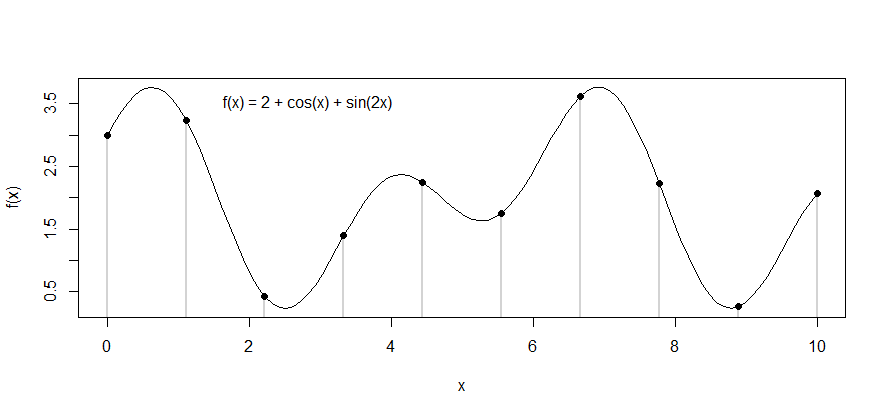
\includegraphics[height = 4.5cm, width = 9cm]{figure_man/simple-comp.png}
\end{figure}
\end{center}

How do we calculate $cos(x)$ here?\\
Possible answer: approximated Taylor series!

\end{vbframe}

\begin{vbframe}{Example: Equation solving / Root finding}

\begin{center}
\begin{figure}
  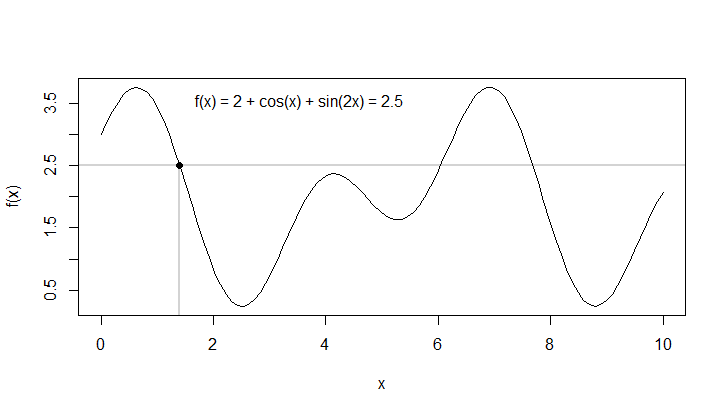
\includegraphics[height = 5cm, width = 9cm]{figure_man/Equation-solving.png}
\end{figure}
\end{center}

\framebreak

For a tolerance of $0.001$, the numerical solution is:

%<<include=FALSE>>=
%opts_chunk$set(size = "scriptsize")
%@
\footnotesize
\begin{verbatim}
f = function(x) { 2 + cos(x) + sin(2 * x) }
f0 = function(x) { f(x) - 2.5 }
uniroot(f0, c(0, 4), tol = 0.001)
## $root
## [1] 1.401727
##
## $f.root
## [1] -2.382814e-06
##
## $iter
## [1] 6
##
## $init.it
## [1] NA
##
## $estim.prec
## [1] 0.0005500599
\end{verbatim}


\end{vbframe}

% \begin{vbframe}{Example for an Identification Problem}

% \begin{center}
% <<echo = FALSE>>=
% set.seed(111)
% x2 = x
% x = seq(0, 10, length = 30)
% e = rnorm(length(x), sd = 0.2)
% y = f(x) + e
% plot(y ~ x, ylab = "y")
% text(1.5, 3.5, expression(y == 2 + cos(x) + sin(2 * x) + epsilon), pos = 4)
% b = lm(y ~ 1 + poly(x, 11))
% @
% \end{center}

% \framebreak

% Polynomial of degree $11$:
% $$
% y = \beta_0 + \beta_1x + \beta_2x^2 + \ldots + \beta_{11}x^{11} + \varepsilon
% $$

% \lz

% Estimated coefficients:

% <<echo=FALSE>>=
% cb <- coef(b)
% names(cb) = paste("x^", 0:11, sep = "")
% print(cb)
% @

% \lz

% Error (standard deviation) on the sample: round(summary(b)$sigma, 4)

% \framebreak

% \begin{center}
% <<echo = FALSE>>=
% plot(y ~ x, ylab = "y")
% text(1.5, 3.5, expression(y == 2 + cos(x) + sin(2 * x) + epsilon), pos = 4)
% fit = predict(b, newdata = list(x = x2))
% lines(fit ~ x2)
% @

% \end{center}

% % \framebreak

% % \begin{itemize}
% %   \item For a linear model, the variance of the estimator and thus the variance of the predicted values can, under certain assumptions, be calculated in closed-form:

% %   $$
% % \hat{\boldsymbol{\beta}} \sim N(\boldsymbol{\beta},
% %     \sigma^2 (\mathbf{X}^{\top}\mathbf{X})^{-1} / N)
% %   $$
% %   $$
% % \hat{y}_0 \sim N(y_0,
% %     \sigma^2 \mathbf{x}_0^\top(\mathbf{X}^{\top}\mathbf{X})^{-1}\mathbf{x}_0 / N)
% %   $$
% %   \item What happens if the assumptions do not apply?
% %   \item How large is the variation in a non-parametric smoothing?
% %   \end{itemize}

% \end{vbframe}

% \framebreak

% \begin{center}
% <<echo = FALSE, fig.keep='all'>>=
% fit0 = fitted(b)
% fb = NULL
% for(i0 in 1:100) {
%   ys = fit0 + rnorm(length(x), sd = b$s)
%   bb = loess(ys ~ x, span = 0.33)
%   fb = cbind(fb, predict(bb, newdata = data.frame(x = x2)))
% }
% fit = t(apply(fb, 1, function(x) {
%  c(quantile(x, prob = 0.0275), mean(x), quantile(x, prob = 0.975))
% }))
% plot(y ~ x, ylab = "y", ylim = (ylim <- range(c(y, fit))))
% matplot(x2, fit, type = "l", lty = c(2, 1, 2), col = "black", add = TRUE)
% @
% \end{center}

% Idee: Schätze Modell wiederholt aus verschiedenen Datensätzen,
% betrachte Schwankungen der resultierenden Schätzer:
% \begin{enumerate}
% \item Passe Modell $y_i = f(x_i) + \epsilon_i$ an Daten an: schätze
%   Koeffizienten $\hat{\boldsymbol{\beta}}$ und Fehlervarianz $\hat{\sigma}^2$.
% \item Erzeuge neue Responses:
% $$
% \tilde y_i = \hat{f}(x_i) + \tilde{\varepsilon}_i, \qquad
%   \tilde{\varepsilon}_i\sim N(0, \hat{\sigma}^2)
%   $$
% \item Passe Modell an neue Daten $\{(x_1, \tilde{y}_1), \ldots, (x_n, \tilde{y}_n)\}$ an.
% \item Wiederhole ab~2 (z.B.\ 100 Mal).
% \item Evaluiere Schwankungen der Koeffizienten, Prognose, usw.
% \end{enumerate}

% \framebreak

% \begin{center}
% <<echo = FALSE, fig.keep='all'>>=
% plot(y ~ x, ylab = "y", ylim = ylim)
% points(x, ys, col = "blue")
% lines(fb[, 100] ~ x2, col = "blue")
% matplot(x2, fit, type = "l", lty = c(2, 1, 2), col = "black", add = TRUE)
% @
% \end{center}

% \framebreak

% \begin{center}
% <<echo = FALSE, fig.keep='all'>>=
% plot(x, y, ylim = ylim)
% matplot(x2, fb, type = "l", lty = 1, col = rgb(0.1, 0.1, 0.1, alpha = 0.1), add = TRUE)
% lines(f(x2) ~ x2, col = "red")
% @
% \end{center}
% \end{vbframe}


% \begin{vbframe}{Parametrischer Bootstrap}

% Das vorgestellte Verfahren heißt \enquote{parametrischer Bootstrap}.

% Zutaten:
% \begin{itemize}
% \item eine programmierbare Umgebung für statistisches Rechnen
% \item das Verfahren selber (hier: LOESS), inkl.~Berechnung
%   prognostizierter Werte
% \item ein Generator für normalverteilte Zufallszahlen
% \end{itemize}
%
% \framebreak
%
% Code:
%
%  <<echo = TRUE, eval = FALSE>>=
%  b = loess(y ~ x, span = 0.33)
%  fit0 = fitted(b)
% fb = NULL
% for(i in 1:100) {
%   ys = fit0 + rnorm(length(x), sd = b$s)
%   bb = loess(ys ~ x, span = 0.33)
%   fb = cbind(fb, predict(bb))
% }
% fit = apply(fb, 1, function(x) {
%   quantile(x, prob = c(0.0275, 0.5, 0.975))
% })
% @
%
%
% \end{vbframe}
\normalsize
\begin{vbframe}{Example: Sampling}

How does a computer generate randomness?
How does \texttt{R} calculate:
\lz
\footnotesize
\begin{verbatim}
rnorm(10)
## [1] 0.06758659 0.67908219 -0.26783828 0.77266612
## [5] -0.02887604 -0.46867480 -0.94277461 0.15943498
## [9] -0.73383393 -0.48259188
\end{verbatim}


\normalsize
\lz
\begin{itemize}
\item How do we sample from a "non-standard" density?
\item Wait for someone to create a CRAN package for it...?
\end{itemize}

\end{vbframe}

\begin{vbframe}{Example: Linear Model}

How do we solve the normal equations?

  $$ \bm{\beta} = \olsest $$

\begin{itemize}
\item So invert matrix once (how does that work?),
  then 2 matrix multiplications? Nope! See chapter on matrix decompositions.
\item How exact is that?
\item How expensive is it for large $n$?
\end{itemize}

\end{vbframe}

\begin{vbframe}{Example: LASSO}
 How do we optimize something like this?
  $$\sumin (\bm{\beta}^T \xv^{(i)} - y^{(i)})^2 + \lambda \sumjp |\beta_j|$$

  \begin{itemize}
    \item Analytically solvable? Answer: no!
    \item How does it work "numerically"?
    \item How expensive is it?
  \end{itemize}
\end{vbframe}

%\end{frame}


\endlecture
\end{document}
